% Options for packages loaded elsewhere
\PassOptionsToPackage{unicode}{hyperref}
\PassOptionsToPackage{hyphens}{url}
\documentclass[
  ignorenonframetext,
]{beamer}
\newif\ifbibliography
\usepackage{pgfpages}
\setbeamertemplate{caption}[numbered]
\setbeamertemplate{caption label separator}{: }
\setbeamercolor{caption name}{fg=normal text.fg}
\beamertemplatenavigationsymbolsempty
% remove section numbering
\setbeamertemplate{part page}{
  \centering
  \begin{beamercolorbox}[sep=16pt,center]{part title}
    \usebeamerfont{part title}\insertpart\par
  \end{beamercolorbox}
}
\setbeamertemplate{section page}{
  \centering
  \begin{beamercolorbox}[sep=12pt,center]{section title}
    \usebeamerfont{section title}\insertsection\par
  \end{beamercolorbox}
}
\setbeamertemplate{subsection page}{
  \centering
  \begin{beamercolorbox}[sep=8pt,center]{subsection title}
    \usebeamerfont{subsection title}\insertsubsection\par
  \end{beamercolorbox}
}
% Prevent slide breaks in the middle of a paragraph
\widowpenalties 1 10000
\raggedbottom
\AtBeginPart{
  \frame{\partpage}
}
\AtBeginSection{
  \ifbibliography
  \else
    \frame{\sectionpage}
  \fi
}
\AtBeginSubsection{
  \frame{\subsectionpage}
}
\usepackage{iftex}
\ifPDFTeX
  \usepackage[T1]{fontenc}
  \usepackage[utf8]{inputenc}
  \usepackage{textcomp} % provide euro and other symbols
\else % if luatex or xetex
  \usepackage{unicode-math} % this also loads fontspec
  \defaultfontfeatures{Scale=MatchLowercase}
  \defaultfontfeatures[\rmfamily]{Ligatures=TeX,Scale=1}
\fi
\usepackage{lmodern}
\ifPDFTeX\else
  % xetex/luatex font selection
\fi
% Use upquote if available, for straight quotes in verbatim environments
\IfFileExists{upquote.sty}{\usepackage{upquote}}{}
\IfFileExists{microtype.sty}{% use microtype if available
  \usepackage[]{microtype}
  \UseMicrotypeSet[protrusion]{basicmath} % disable protrusion for tt fonts
}{}
\makeatletter
\@ifundefined{KOMAClassName}{% if non-KOMA class
  \IfFileExists{parskip.sty}{%
    \usepackage{parskip}
  }{% else
    \setlength{\parindent}{0pt}
    \setlength{\parskip}{6pt plus 2pt minus 1pt}}
}{% if KOMA class
  \KOMAoptions{parskip=half}}
\makeatother
\usepackage{longtable,booktabs,array}
\usepackage{caption}
\captionsetup[table]{skip=6pt}
\newcounter{none} % for unnumbered tables
\usepackage{calc} % for calculating minipage widths
\usepackage{caption}
% Make caption package work with longtable
\makeatletter
\def\fnum@table{\tablename~\thetable}
\makeatother
\usepackage{graphicx}
\makeatletter
\newsavebox\pandoc@box
\newcommand*\pandocbounded[1]{% scales image to fit in text height/width
  \sbox\pandoc@box{#1}%
  \Gscale@div\@tempa{\textheight}{\dimexpr\ht\pandoc@box+\dp\pandoc@box\relax}%
  \Gscale@div\@tempb{\linewidth}{\wd\pandoc@box}%
  \ifdim\@tempb\p@<\@tempa\p@\let\@tempa\@tempb\fi% select the smaller of both
  \ifdim\@tempa\p@<\p@\scalebox{\@tempa}{\usebox\pandoc@box}%
  \else\usebox{\pandoc@box}%
  \fi%
}
% Set default figure placement to htbp
\def\fps@figure{htbp}
\makeatother
\setlength{\emergencystretch}{3em} % prevent overfull lines
\providecommand{\tightlist}{%
  \setlength{\itemsep}{0pt}\setlength{\parskip}{0pt}}
% Auto-generated by infrastructure/rendering/_pdf_latex_helpers.py::extract_math_font_preamble.
% Minimal header passed to Pandoc via -H so Beamer slides pick up the same math font
% as the combined-PDF path. Adjust the manuscript's preamble.md to change the font globally.
\usepackage{unicode-math}
\setmathfont{latinmodern-math.otf}

% Slide layout defaults for warning-clean scientific decks.
\usepackage{etoolbox}
\IfFileExists{xurl.sty}{\usepackage{xurl}}{}
\IfFileExists{seqsplit.sty}{\usepackage{seqsplit}}{\newcommand{\seqsplit}[1]{#1}}
\protected\def\breakseq#1{\seqsplit{#1}}
\protected\def\breaktt#1{\begingroup\ttfamily\seqsplit{#1}\endgroup}
\setlength{\emergencystretch}{6em}
\tolerance=5000
\hbadness=10000
\hfuzz=1pt
\setlength{\tabcolsep}{2pt}
\AtBeginEnvironment{longtable}{\tiny\renewcommand{\arraystretch}{0.86}\setlength{\tabcolsep}{1pt}}
\AtBeginEnvironment{tabular}{\tiny\renewcommand{\arraystretch}{0.86}\setlength{\tabcolsep}{1pt}}
\AtBeginEnvironment{equation}{\tiny}
\AtBeginEnvironment{equation*}{\tiny}
\AtBeginEnvironment{align}{\tiny}
\AtBeginEnvironment{align*}{\tiny}
\AtBeginEnvironment{itemize}{\footnotesize}
\AtBeginEnvironment{enumerate}{\footnotesize}
\AtBeginEnvironment{description}{\footnotesize}
\setbeamerfont{caption}{size=\tiny}
\setbeamerfont{caption name}{size=\tiny}
\setbeamerfont{normal text}{size=\small}
\setbeamerfont{frametitle}{size=\small}
\setbeamerfont{section title}{size=\footnotesize}
\setbeamerfont{subsection title}{size=\footnotesize}
\setbeamertemplate{section page}{%
  \centering
  \begin{beamercolorbox}[sep=12pt,center,wd=\paperwidth]{section title}
    \parbox{0.86\paperwidth}{\centering\usebeamerfont{section title}\insertsection\par}
  \end{beamercolorbox}
}
\setbeamertemplate{subsection page}{%
  \centering
  \begin{beamercolorbox}[sep=8pt,center,wd=\paperwidth]{subsection title}
    \parbox{0.86\paperwidth}{\centering\usebeamerfont{subsection title}\insertsubsection\par}
  \end{beamercolorbox}
}
\setlength{\abovecaptionskip}{2pt}
\setlength{\belowcaptionskip}{0pt}

% Natbib and cross-reference fallbacks — slides don't load natbib
% or cleveref, but combined-PDF manuscript prose may emit these
% commands. The fallback renders citations as a bracketed key list
% and cross-references as detokenized labels so slides don't fail on
% undefined control sequences or raw underscores. \providecommand is
% a no-op if packages load later.
\providecommand{\citep}[1]{[#1]}
\providecommand{\citet}[1]{#1}
\providecommand{\citealp}[1]{#1}
\providecommand{\citeauthor}[1]{#1}
\providecommand{\citeyear}[1]{#1}
\providecommand{\cref}[1]{\texttt{\detokenize{#1}}}
\providecommand{\Cref}[1]{\texttt{\detokenize{#1}}}

% Pandoc's article template uses codelisting floats for captioned code; Beamer has no such float, so provide a slide-safe numbered block.
\newcounter{codelisting}
\renewcommand{\thecodelisting}{\arabic{codelisting}}
\newenvironment{codelisting}{%
  \refstepcounter{codelisting}%
  \begin{center}\begin{minipage}{0.96\linewidth}\footnotesize%
  \renewcommand{\caption}[1]{\par\smallskip\textbf{Listing~\thecodelisting: }##1\par\smallskip}%
}{%
  \end{minipage}\end{center}%
}
\newtheorem{proposition}{Proposition}
\newtheorem{hypothesis}{Hypothesis}
\usepackage{bookmark}
\IfFileExists{xurl.sty}{\usepackage{xurl}}{} % add URL line breaks if available
\urlstyle{same}
% fallback for those not using the hyperref driver hyperxmp:
\makeatletter
\@ifundefined{xmpquote}{\newcommand{\xmpquote}[1]{#1}}{}
\makeatother
\hypersetup{
  hidelinks,
  pdfcreator={LaTeX via pandoc}}

\author{\texorpdfstring{}{}}
\date{}

\begin{document}

\section{Parameter recovery: acuity selection on the tested
grid}\label{sec:results-parameter-recovery}

\begin{frame}[allowframebreaks]{Parameter recovery: acuity selection on
the tested grid}
Parameter recovery probes whether the executed observation model
contains enough information to distinguish sensor acuity under the study
design. We sweep acuity values 0.60, 0.70, 0.80, 0.90: for each true
acuity the model generates 200 synthetic observations per trial across
960 independent trials, fits acuity by marginal-likelihood grid search,
and compares the recovered value with ground truth.

Across the sweep the mean absolute recovery error is 0.0232 and the
coefficient of determination of mean-recovered versus true acuity is
\(R^2\) = 0.9999. Within this finite grid and observation budget,
recovered acuity tracks the identity line with the reported error
(fig.~\ref{fig:parameter-recovery}). This is evidence of practical
acuity recoverability for the executed design, not a proof of global or
structural identifiability and not an acuity-by-colony-size study.

\end{frame}

\begin{frame}[allowframebreaks]{Parameter recovery: acuity selection on
the tested grid}
\begin{figure}
\centering
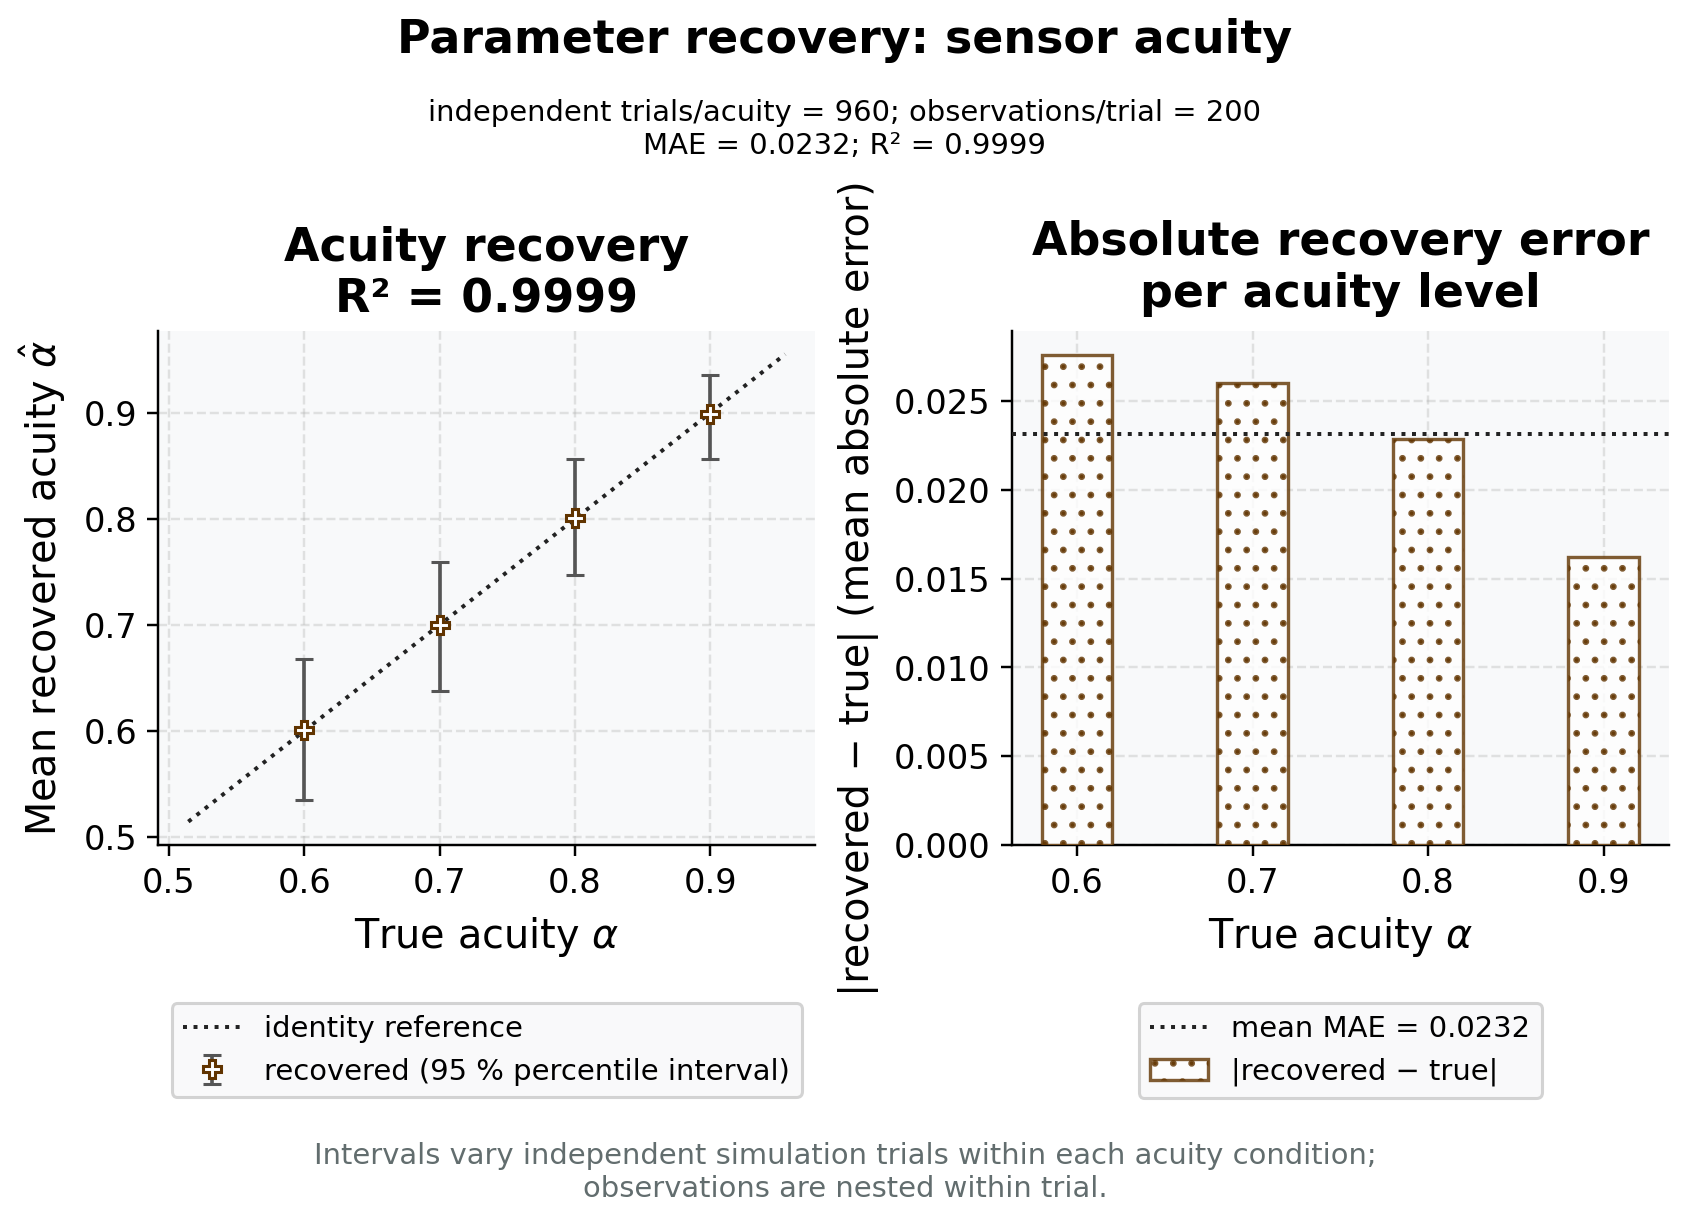
\includegraphics[width=0.9\linewidth,height=0.40\textheight,keepaspectratio,alt={Two-panel parameter-recovery figure. Source relation: original project parameter-recovery diagnostic; estimand: recovered acuity and absolute error in probability units; uncertainty: empirical percentile intervals across independent trials. In the left panel, the x-axis is true acuity and the y-axis is recovered acuity, both in probability units; error bars show the 95\% empirical percentile interval across 960 trials per condition, and the diagonal is the identity reference. This interval is a descriptive quantile of the independent-trial estimates, not a bootstrap confidence interval or Bayesian credible interval. In the right panel, the x-axis is tested true acuity and the y-axis is absolute acuity error in probability units; the horizontal line is the global mean absolute error. These finite-grid results quantify acuity recovery for 200 observations per trial; they do not establish global structural identifiability.}]{../figures/parameter_recovery.png}
\caption{Two-panel parameter-recovery figure. Source relation: original
project parameter-recovery diagnostic; estimand: recovered acuity and
absolute error in probability units; uncertainty: empirical percentile
intervals across independent trials. In the left panel, the x-axis is
true acuity and the y-axis is recovered acuity, both in probability
units; error bars show the 95\% empirical percentile interval across 960
trials per condition, and the diagonal is the identity reference. This
interval is a descriptive quantile of the independent-trial estimates,
not a bootstrap confidence interval or Bayesian credible interval. In
the right panel, the x-axis is tested true acuity and the y-axis is
absolute acuity error in probability units; the horizontal line is the
global mean absolute error. These finite-grid results quantify acuity
recovery for 200 observations per trial; they do not establish global
structural identifiability.}\label{fig:parameter-recovery}
\end{figure}
\end{frame}

\end{document}
